
Initially the system performance requirements were defined. It should be noted however that the team could not manage to meet some of these requirements within the project timeline, specifically OR01, and ER03.
\subsection{System requirements}
\textbf{FR01}: The rotator must be able to move the antenna around the vertical and lateral axis.\\
\textbf{FR02}: The rotator should have a pointing accuracy of $2\degree$.\\
\textbf{FR03}: The rotator should be able to accelerate at $10\degree/s²$ max.\\
\textbf{FR04}: The rotator must have a directional velocity of $5\degree/s$ typical to $20\degree$ max.\\
\textbf{OR01}: The rotator must be able to automatically track satellites.\\
\textbf{ER01}: The rotator must be able to withstand temperatures between $-10\degree C$ and $+40\degree C$.\\
\textbf{ER02}: The rotator must be able to withstand wind loads up to 25 km/s.\\
\textbf{ER03}: The rotator shielding must be able to block rain capacities up to 5 cm/hr.\\
\textbf{LR01}: The rotator must be installable within 10 minutes on site.\\
\textbf{DR01}: The rotator mounting shall be adaptable to standard 35 mm tripod masts.\\
\\
FR: Functional Requirements, OR: Operational Requirements, LR: Logistics Support Requirements, ER: Environmental Requirements, DR: Design Requirement.

\subsection{Work breakdown structure}
The flow of work is subdivided into three main technical branches and the final documentation.
\begin{figure}[H]
	\centering
	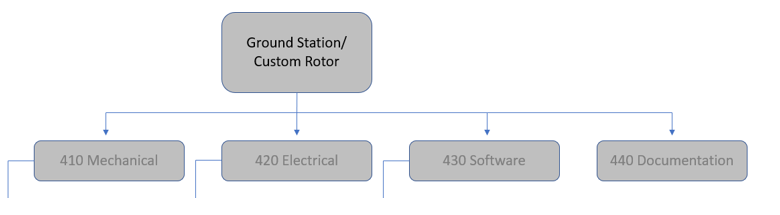
\includegraphics[width=0.8\textwidth]{../art/chart.png}
	\caption{Excerpt from WP-400 work breakdown chart.}
\end{figure}